\begin{pastexam}[label={px:ccu-114-csb-09}]{中正資工所乙組 114 學年度 第 9 題}
（單選）

(5\%) Find the vertices in order while performing \textbf{Dijkstra algorithm} on the graph below, starting from source vertex $A$. If two unvisited vertices have the same distance during the algorithm, choose the vertex with the smaller alphabetical order first.

\begin{center}
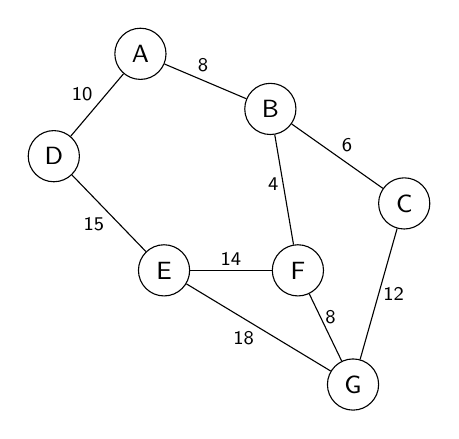
\begin{tikzpicture}[v/.style={circle,draw,minimum size=6.5mm,inner sep=0pt,font=\sffamily\small},w/.style={font=\sffamily\scriptsize,inner sep=1.5pt},x=1cm,y=1cm]
\node[v] (A) at (1.1,4.2) {A};
\node[v] (B) at (2.75,3.5) {B};
\node[v] (D) at (0,2.9) {D};
\node[v] (C) at (4.45,2.3) {C};
\node[v] (E) at (1.4,1.45) {E};
\node[v] (F) at (3.1,1.45) {F};
\node[v] (G) at (3.8,0) {G};
\draw (A)--node[w,above right,pos=0.35]{8}(B);
\draw (A)--node[w,above left]{10}(D);
\draw (B)--node[w,above right]{6}(C);
\draw (B)--node[w,left,pos=0.45]{4}(F);
\draw (D)--node[w,below left]{15}(E);
\draw (E)--node[w,above]{14}(F);
\draw (E)--node[w,below left]{18}(G);
\draw (F)--node[w,right,pos=0.35]{8}(G);
\draw (C)--node[w,right]{12}(G);
\end{tikzpicture}
\end{center}

\begin{enumerate}[label=\Alph*.]
\item (A, D, B, E, F, C, G)
\item (A, B, F, G, C, D, E)
\item (A, D, B, F, G, C, E)
\item (A, B, D, F, C, G, E)
\item None of the above
\end{enumerate}
\end{pastexam}

\begin{pastsoln}
答案是 D（A, B, D, F, C, G, E）。

圖是無向圖，每條邊兩個方向都能走。 照資結書虛擬碼~25.3，起點 A，每輪取出 $d$ 最小的未確定頂點（平手取字母小的），再放鬆它的
鄰邊。 表裡每一列是取出該頂點並放鬆後的 $d$，粗體是這輪取出的頂點，``---'' 表示已確定。
\begin{center}
\small
\begin{tabular}{cc*{7}{c}l}
\toprule
輪 & 取出 & A & B & C & D & E & F & G & 放鬆 \\
\midrule
1 & A & \textbf{0} & 8 & $\infty$ & 10 & $\infty$ & $\infty$ & $\infty$ & A--B、A--D \\
2 & B & --- & \textbf{8} & 14 & 10 & $\infty$ & 12 & $\infty$ & B--C：$8 + 6$；B--F：$8 + 4$ \\
3 & D & --- & --- & 14 & \textbf{10} & 25 & 12 & $\infty$ & D--E：$10 + 15$ \\
4 & F & --- & --- & 14 & --- & 25 & \textbf{12} & 20 & F--E：$26$ 不更新；F--G：$12 + 8$ \\
5 & C & --- & --- & \textbf{14} & --- & 25 & --- & 20 & C--G：$26$ 不更新 \\
6 & G & --- & --- & --- & --- & 25 & --- & \textbf{20} & G--E：$38$ 不更新 \\
7 & E & --- & --- & --- & --- & \textbf{25} & --- & --- & \\
\bottomrule
\end{tabular}
\end{center}
過程中沒有出現平手。 取出順序 A, B, D, F, C, G, E，選 D。 最短距離：A $0$、B $8$、C $14$、D $10$、E $25$、F $12$、G $20$。

逐項檢查：
\begin{itemize}
\item A：第二個取 D（$10$），但 B 是 $8$。 錯。
\item B：B 之後取 F（$12$），但 D 是 $10$；而且 D、E 被排到最後。 錯。
\item C：同 A，第二個不該是 D。 錯。
\item D：上表的順序。 對。
\item E：D 是對的。 錯。
\end{itemize}
\end{pastsoln}
